\part{Diseño de VCO}
\section{Introducción}
En esta sección se busca diseñar e implementar un VCO (\textit{Voltage Controlled Oscilator}) con un rango de trabajo de $0V - 5V$ y que genere una señal senoidal de amplitud $1V$ en un rango de $1kHz$ a $10kHz$.

\section{Introducción teórica}

Muchas aplicaciones requieren tener una frecuencia de salida $f_0$ que se programe automáticamente mediante el control de una tensión $V_I$. Este es el trabajo de un $VCO$, que esta diseñado de modo que devuelve:

\begin{equation}
    f_0 = k V_{IN}
    \label{eq:f0}
\end{equation}

Donde $V_I > 0$ y $k$ es la sensibilidad del $VCO$ con unidades de hertz por volt. 



Los $VCOs$ se pueden dividir en dos grupos:


\textbf{Osciladores armónicos}: la salida del oscilador es senoidal. Estos tipos de osciladores son mas difíciles de implementar pero tienen una mejor estabilidad que el otro tipo de osciladores. También, son llamados osciladores de voltaje lineal. Se pueden implementar con circuitos RC, LC o tanque. En estos tipos de osciladores es importante tener en cuenta el parámetro $THD$ (\textit{total harmonic distortion}) que expresa la pureza de la onda senoidal. Su expresión esta dada por:
    
    \begin{displaymath}
        THD (\%) = 100 \frac{\sqrt{D^2_2 + D^2_3 + D^2_4 + ...}}{D_1}
    \end{displaymath}

    Donde $D_k (k=2,3,4,...)$ es el ratio de la amplitud del armónico $k$ del armónico fundamental de la serie de Fourier de la onda dada. 

    
    \textbf{Osciladores de relajación}: la salida del oscilador es del tipo triangular, diente de cierra, pulso o cuadrada. En general, son mas fáciles de implementar que los osciladores armónicos. 
    
    \begin{wrapfigure}{l}{0.35\textwidth}
        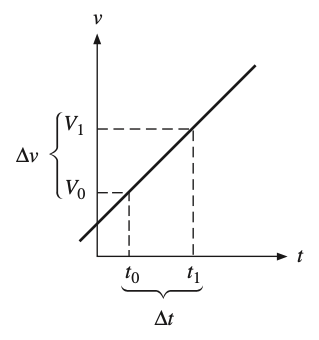
\includegraphics[width=0.9\linewidth]{../Ex3/Resources/lineal_waveform.png}
        \caption{Onda lineal}
        \label{fig:ej3_lineal_waveform}
        \end{wrapfigure}
    
    Para obtener este tipo de salidas se utilizan dispositivos biestables como interruptores, \textit{Schimitt triggers}, compuertas logicas, flip-flops para que rápidamente se pueda cargar y descargar un capacitor.
    

    La descarga y descarga del capacitor es la responsable de dar el tipo de señal de salida. Luego, es de particular interés determinar el $\Delta t$ que le toma al capacitor cargar y descargarse por una determinada cantidad de $\Delta v$. Las formas mas comunes de carga y descarga son la lineal y la exponencial. La primera se da cuando, por el capacitor fluye una corriente constante. Luego, se obtiene una rampa como se ve en la Figura \ref{fig:ej3_lineal_waveform}. Este tipo de función permite estimar  $\Delta t$. Su expresión es:
	\begin{equation}
        \Delta t = \frac{C}{I} \Delta v
        \label{eq:delta_t}
    \end{equation} 

\section{Diseño}

Si bien el objetivo es obtener un $VCO$ cuya salida es una señal senoidal, no se realiza un oscilador armónico sino que se utiliza un oscilador de relajación. Se propone diseñar un oscilador de relajación que devuelva una señal triangular y luego hacer una conversión de dicha triangular a senoidal. En primer lugar se diseña un $VCO$ triangular y luego se diseña un convertor de señal triangular a senoidal. 

\subsection{VCO triangular Parte 1}


\begin{figure}[h!]                                                       
    \centering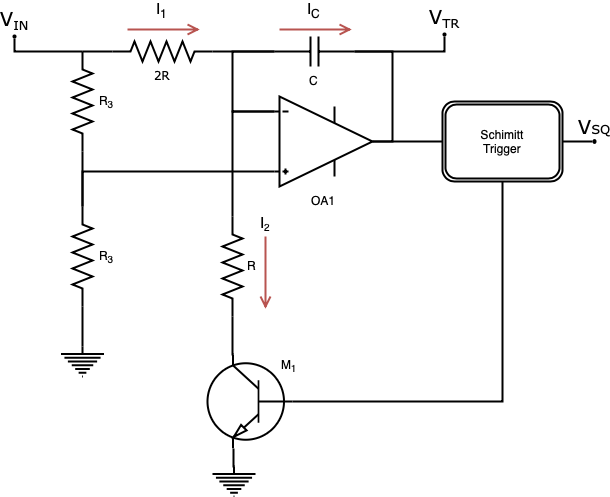
\includegraphics[width=0.6\textwidth]{../Ex3/Resources/circuito_propuesto_1.png}
    \caption{Circuito propuesto VCO}
    \label{fig:VCO_circuito_propuesto_1}
    \end{figure}


Se propone el circuito de la Figura \ref{fig:VCO_circuito_propuesto_1}. Como se puede ver, el mismo cuenta con un \textit{Schimitt trigger} como se anticipo en la sección anterior. La función del trigger es variar la tensión $V_{SQ}$ entre dos valores, $V_{TH}$ (\textit{trigger high}) y $V_{TL}$ (\textit{trigger low}). Esto hace que la señal triangular $V_{TR}$ también varie entre estos dos valores. En consecuencia, como se quiere que la amplitud de la señal con amplitud de $1V$ se define que la diferencia $\Delta V_{TR} = V_{TH} - V_{TL} = 2V$. Mas adelante se analiza como implementar el trigger, por el momento se analiza el resto del circuito.  

El amplificador operacional $OA_1$ es un conversor tension-corriente que fuerza al capacitor $C$ conducir linealmente y proporsional a la tensión de entrada $V_{IN}$. Se debe tener en mente que, como el capacitor se debe cargar y descargar, la corriente que circula por el capacitor $I_C$ se debe alternar entre polaridades opuestas. Ver que, la tensión en ambas terminales de $OA_1$ tienen la misma tensión $\frac{V_{IN}}{2}$ (se considera al amplificador operacional como ideal) . Esto surge del divisor resistivo que forman ambas $R_3$. Ademas, se puede calcular la corriente que fluye por $2R$ que es:

\begin{displaymath}
    I_1 = \frac{V_{IN} - \frac{V_{IN}}{2}}{2R} = \frac{V_{IN}}{4R}
\end{displaymath}

Nótese que, $I_C$ es:

\begin{displaymath}
    I_C = I_1 - I_2
\end{displaymath}

Para explicar el funcionamiento del circuito primero se asume que que $V_{SQ}$ comienza en $V_{TL}$. Esto implica que el transistor $M_1$ esta apagado por lo que toda la corriente $I_1$ fluye en $C$ ($I_2 = 0A$). Luego, $I_C = I_1$. Al fluir desde la terminal inversora de $OA_1$ hacia su salida de, el capacitor se descarga. Al descargarse, genera una rampa descendiente llevando a $V_{TR} = V_{TL}$. 

Por otro lado, cuando $V_{TR} = V_{TL}$ el tigger \textit{Schimitt} cambia de modo que, $V_{SQ} = V_{TH}$. Esto hace que $M_1$ se encienda poniendo en corto a $R$. Esto implica que $I_2 = \frac{\frac{V_{IN}}{2}}{R} = 2 I_1$. En consecuencia, $I_C = -I_1$. Tomando este sentido, la corriente $I_C$ fluye desde la salida de $OA_1$ hacia la terminal no inversora del mismo, cargando al capacitor y formando una rampa ascendente que lleva a $V_{TR} = V_{TH}$.  

Se puede ver claramente como la corriente del capacitor cambia de sentido formando una señal triangular. A lo largo de todo el ciclo, $I_C$ tiene la expresión:

\begin{equation}
    I_C = \pm \frac{V_{IN}}{4R}
    \label{eq:ic}
\end{equation}



Cuando $V_{TR}$ llega a $V_{TH}$ el tigger vuelve a poner a $V_{SQ}$ en $V_{TL}$, apagando a $M_1$ y comenzando nuevamente el ciclo (oscila). Esto se ve explícitamente en la expresión de $V_{TR}$. Utilizando (\ref{eq:delta_t}) y (\ref{eq:ic}), la expresión de $V_{TR}$ es:


\begin{displaymath} \Delta t = \frac{C}{I_C} \Delta V_C  \end{displaymath}
\begin{displaymath} \Delta V_C = \pm \frac{V_{IN}}{4RC} \Delta t  \end{displaymath}
\begin{displaymath} V_{TR} = \frac{V_{IN}}{2} + V_C \end{displaymath}

\begin{equation}
     V_{TR} = \frac{V_{IN}}{2} \pm \frac{V_{IN}}{4RC} \Delta t 
    \label{eq:v_tr}
\end{equation}


Esta expresión es muy importante ya que muestra la forma que adquiere $V_{TR}$. Ademas, se puede obtener la variación de $V_{TR}$, $\Delta V_{TR}$. De \ref{eq:v_tr}:

\begin{displaymath} \Delta V_{TR} = \frac{V_{IN}}{4RC} \Delta t = \Delta V_C  \end{displaymath}

A su vez, se vio que $V_{TR}$ varia entre las tensiones del trigger. Luego:

\begin{displaymath} \Delta V_{TR} = \Delta V_{C} = V_{TH} - V_{TL} \end{displaymath}



Con estas ultimas expresiones y teniendo en cuenta (\ref{eq:delta_t}) y (\ref{eq:ic}), se puede calcular la frecuencia de oscilación $f_0$:


\begin{displaymath} \Delta t = \frac{C}{I_C} \Delta V_C = \frac{T}{2} \end{displaymath}
\begin{displaymath} f_0 = \frac{1}{T} \end{displaymath}


\begin{equation}
    f_0 = \frac{V_{IN}}{8RC (V_{TH} - V_{TL})}
    \label{eq:f0_vco}
\end{equation}

También se puede calcular la sensibilidad $k$ del oscilador. Teniendo (\ref{eq:f0}) y (\ref{eq:f0_vco}):

\begin{equation}
    k = \frac{1}{8RC(V_{TH} - V_{TL})}
    \label{eq:k}
\end{equation}

Como se puede observar, las ecuaciones halladas dependen de $V_{TH}$ y $V_{TL}$ por lo que a continuación se diseña el tigger.


\subsection{Schimmit trigger}

%pagina 451 franco
\begin{wrapfigure}{r}{0.3\textwidth}
    \begin{center}
        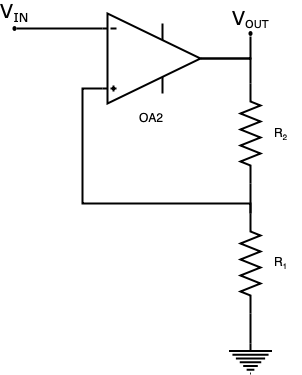
\includegraphics[scale = 0.5]{../Ex3/Resources/trigger.png}    
        \caption{Schmitt trigger}  
        \label{fig:ej3_trigger}
    \end{center}
      
    \end{wrapfigure}

   

 Los trigger Schimitt son amplificadores operacionales cuya realimentacion es positiva. Al tener una realimentacion positiva, los amplificadores son forzados hacia la saturación estableciendo dos estados en su salida, $V_{OH}$ y $V_{OL}$. 



  

Se propone el trigger en configuración inversora de la Figura \ref{fig:ej3_trigger} para usar en el diseño del $VCO$. De la figura se puede ver que se utiliza un divisor de tensión para realizar la realimentacion positiva. Como la salida $V_{OUT}$ solo puede tener dos valores posibles, $V_{TH}$ y $V_{TL}$ adquieren las siguientes expresiones:

\begin{equation}
    V_{TH} = \frac{R_1}{R_1 + R_2} V_{OH}
    \label{eq:vth}
\end{equation}

\begin{equation}
    V_{TL} = \frac{R_1}{R_1 + R_2} V_{OL}
    \label{eq:vtl}
\end{equation}

El circuito funciona de la siguiente manera. Para $V_{IN}<<0$, el amplificador operacional satura en $V_{OH}$ y la tensión en la terminal inversora es $V_P = V_{TH}$. Si se aumenta $V_{IN}$ hasta $V_{TH}$, la acción regenerativa de la alimentación positiva hace que $V_{OUT}$ pase de $V_{OH}$ a $V_{OL}$ tan rápido como el amplificador operacional lo permita. 

Esto provoca que $V_P$ pase de $V_{TH}$ a $V_{TL}$. Para cambiar el estado de $V_{OUT}$, se debe bajar $V_{IN}$ hasta que $V_P = V_{TL}$. En este punto, $V_{OUT}$ cambia nuevamente a $V_{OH}$. Este ciclo se puede apreciar con facilidad en la Figura \ref{fig:ej3_VTC}. Como se puede ver, el gráfico muestra uns histeresis con un ancho $\Delta V_T$. Su expresión es:

\begin{equation}
    \Delta V_T = V_{TH} - V_{TL}= \frac{R_1}{R_1 + R_2} (V_{OL} - V_{OL})
    \label{eq:vt}
\end{equation}


\begin{wrapfigure}{l}{0.3\textwidth}
    \begin{center}
        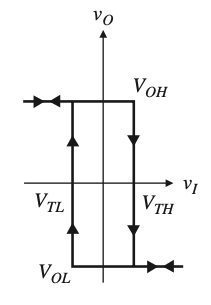
\includegraphics[width=0.65\linewidth]{../Ex3/Resources/vtc.png}  
        \caption{VTC}
        \label{fig:ej3_VTC} 
    \end{center}
\end{wrapfigure}
 
 


Con esta ultima expresión es posible continuar con el diseño del $VCO$. Como se desea que $V_{TH} = 1V$ y $V_{OL} = -1V$, $\Delta V_T = 2$. Sin embargo, para poder darle valores a $R_1$ y $R_2$ se necesita conocer la tensión a la cual el amplificador operacional satura. Esto no se puede conocer a priori pero se puede suponer un valor aproximado para hacer los cálculos. Si se alimenta al amplificador operacional con $\pm 15$ y se presupone que satura en aproximadamente en $\pm 13$, $V_{OH} = 13V$ y $V_{OL} = -13V$. Luego, se llega a la siguiente relación de $R_1$ y $R_2$:

\begin{equation}
    R_2 = 12 R_1
    \label{eq:R_1yR_2}
\end{equation}

Ya es posible darle valores a $R_1$ y $R_2$. Se utilizan los siguientes:

\begin{displaymath}
    R_1 = 1.8k \Omega
\end{displaymath}
\begin{displaymath}
    R_2 = 21.6k \Omega
\end{displaymath}

Para el caso de $R_2$, se utiliza un preset de $25k\Omega$ en lugar del valor obtenido ya que la tensión de saturación puede que no sea $\pm 13V$ y se deba ajustar la resistencia para compensar el error de la tensión de saturación. 

En la Figura \ref{fig:sim_trigger} se puede apreciar una simulación del tigger con los componentes seleccionados. Cabe aclarar que se utilizo el amplificador operacional TL084 para hacer la simulación. Nótese como la tensión de salida toma solo dos estados. Habiendo diseñado satisfactoriamente el trigger ya es posible continuar con el diseño del $VCO$.


\begin{figure}[h!]                                                       
    \centering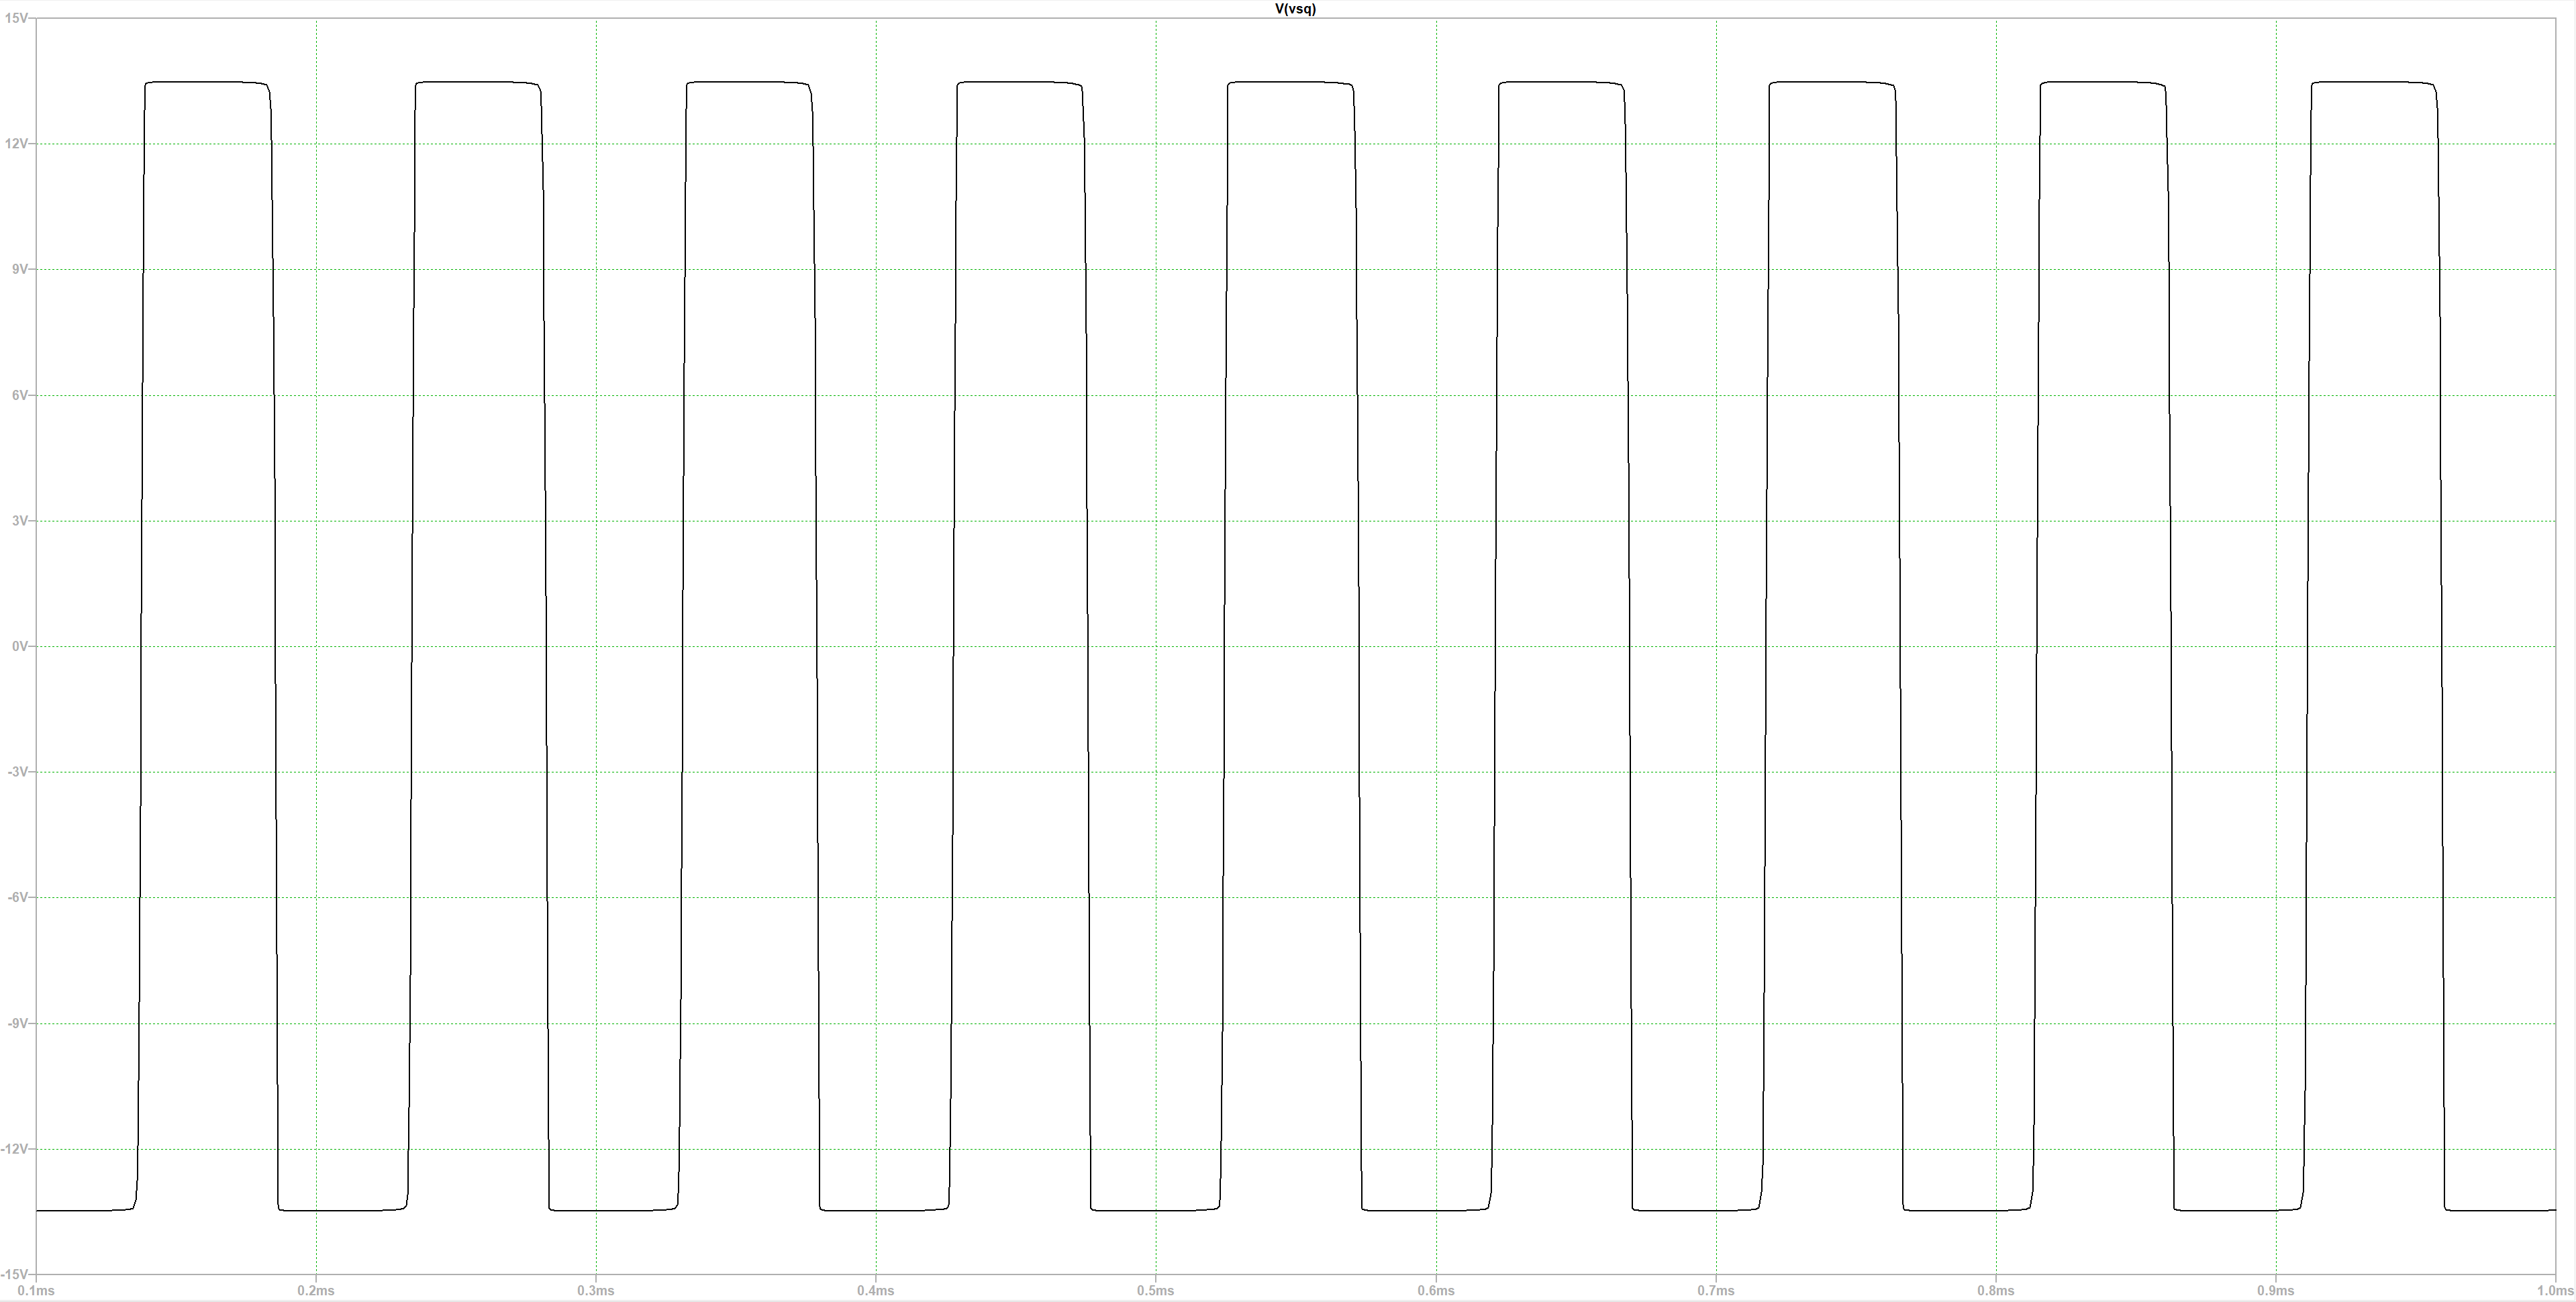
\includegraphics[width=0.9\textwidth]{../Ex3/Resources/sim_trigger.png}
    \caption{Simulación del trigger}
    \label{fig:sim_trigger}
    \end{figure}


\subsection{VCO triangular Parte 2}

\begin{figure}[h!]                                                       
    \centering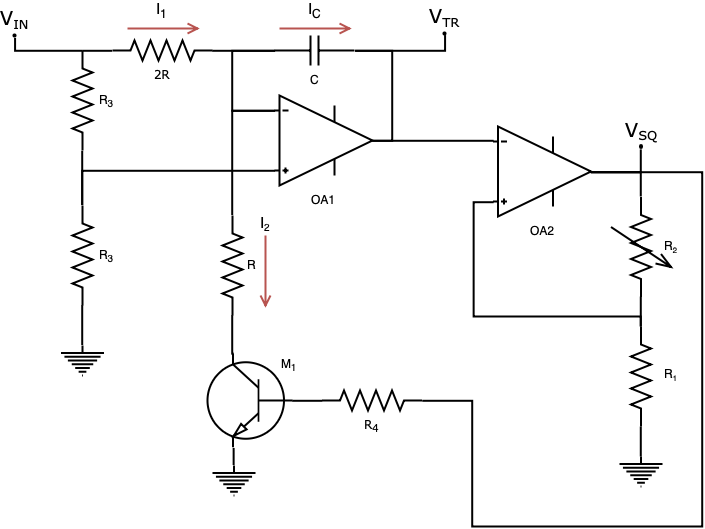
\includegraphics[width=0.7\textwidth]{../Ex3/Resources/circuito_propuesto_2.png}
    \caption{Circuito propuesto}
    \label{fig:VCO_circuito_propuesto_2}
    \end{figure}

\begin{figure}[h!]                                                       
    \centering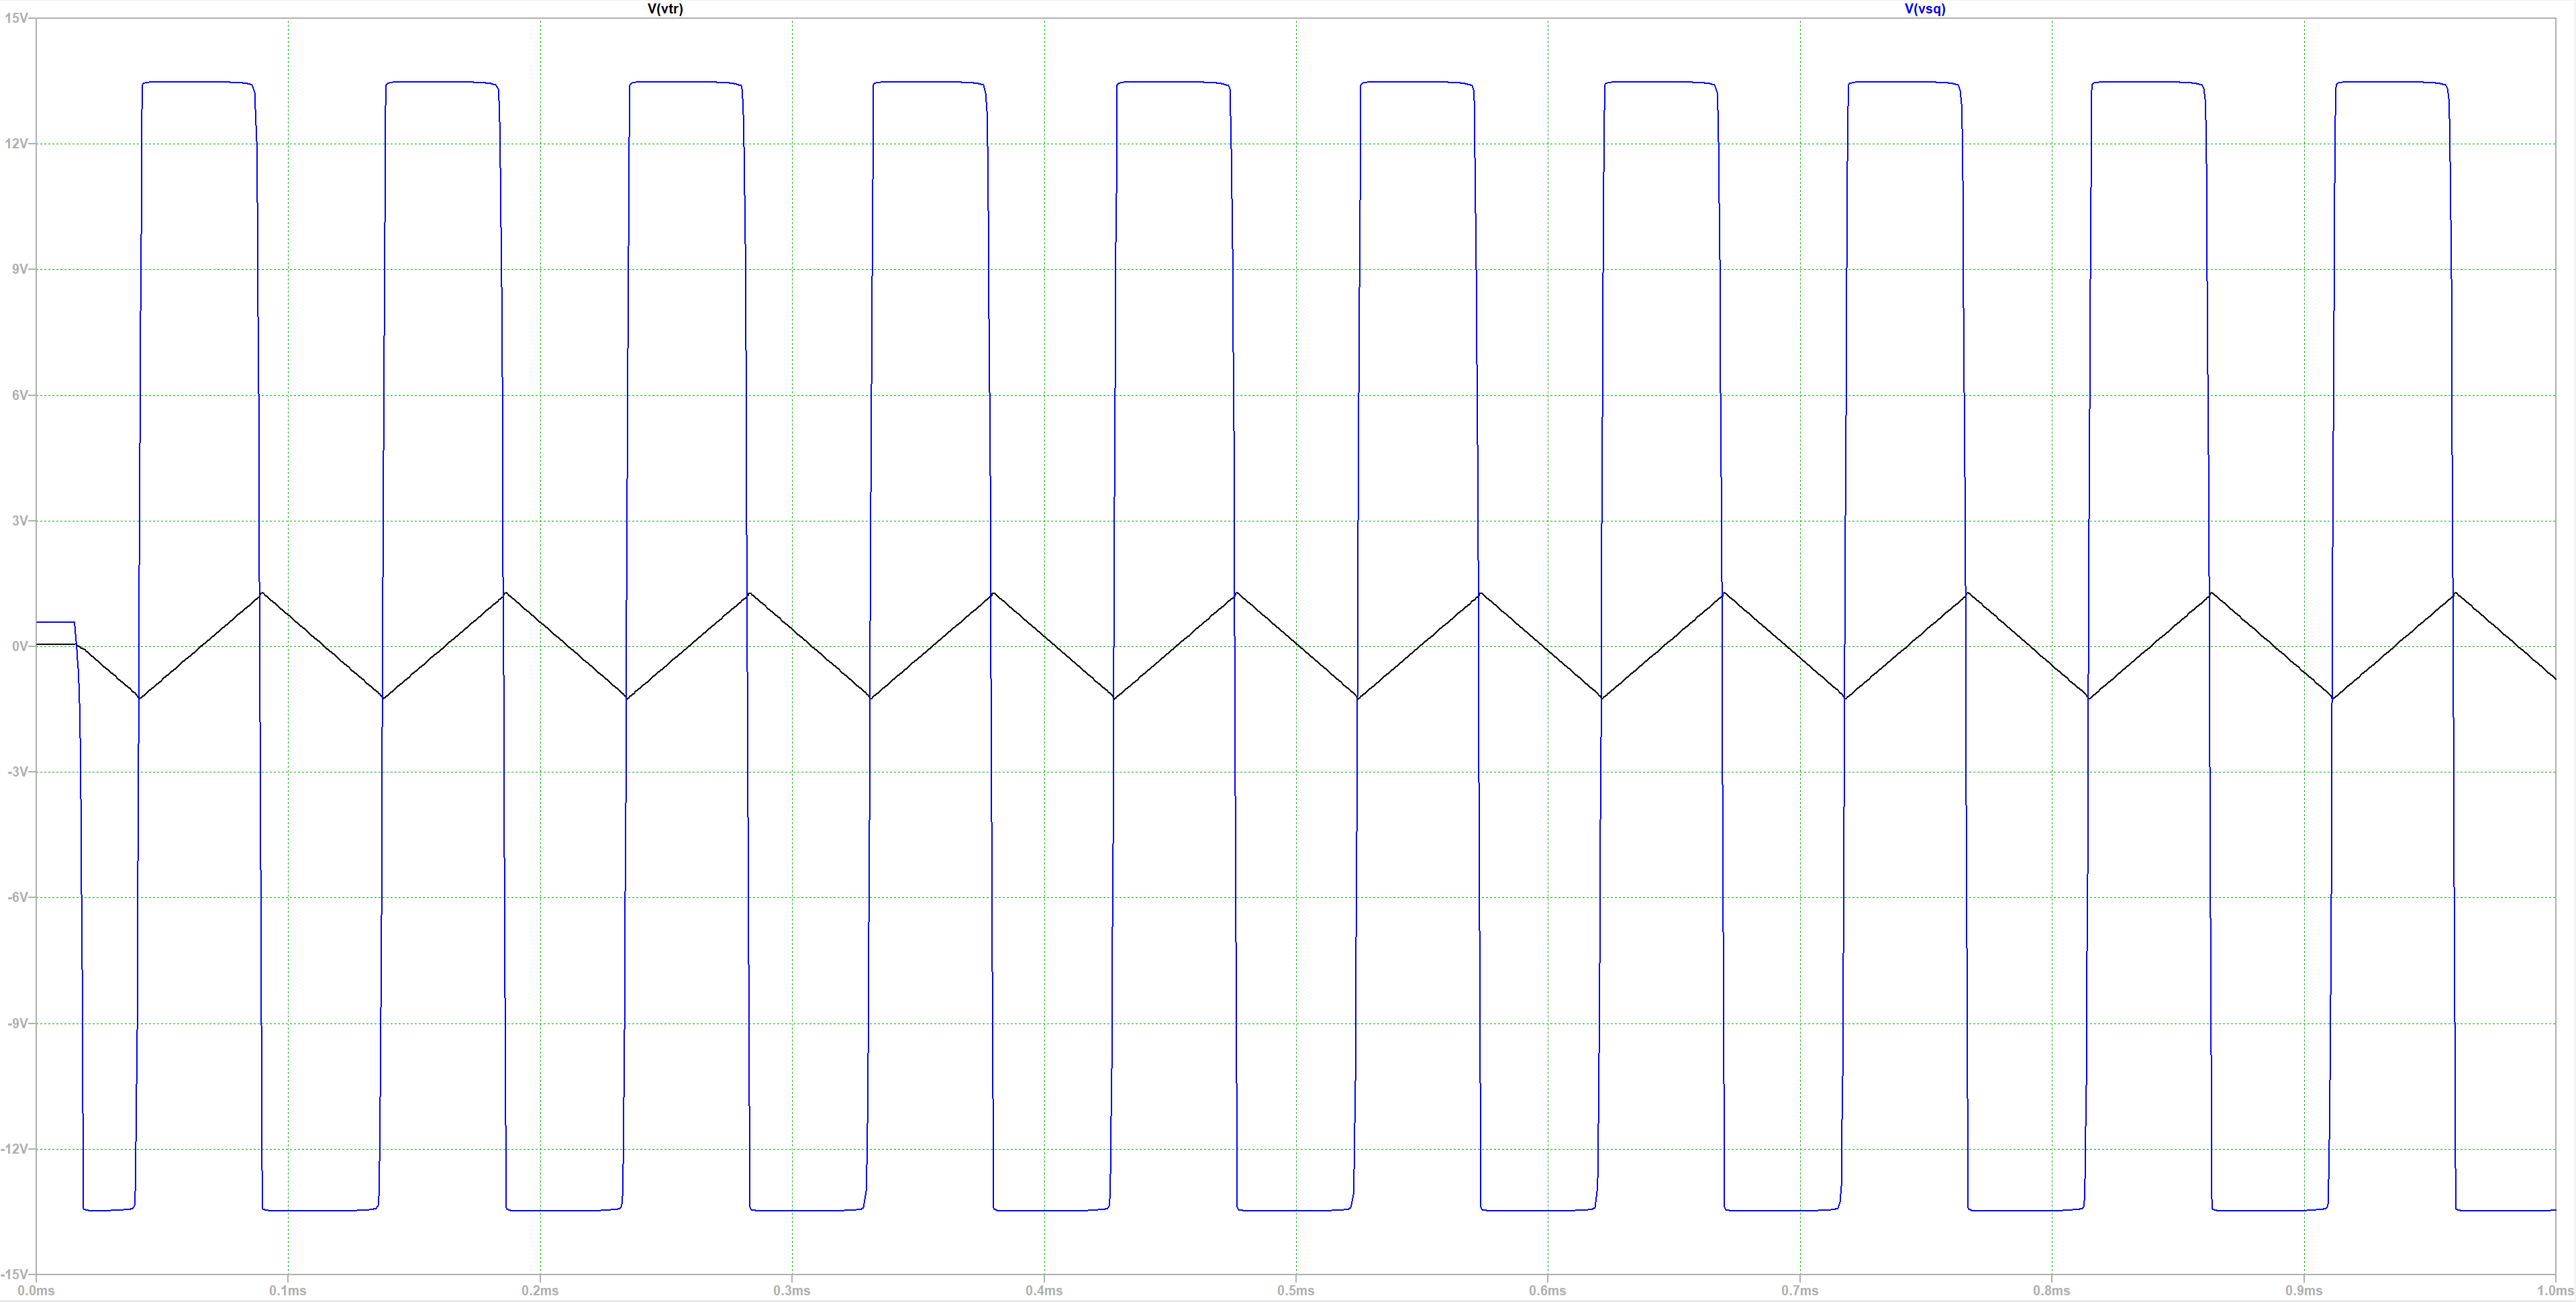
\includegraphics[width=0.9\textwidth]{../Ex3/Resources/sim_vco.png}
    \caption{Simulación del VCO}
    \label{fig:sim_VCO}
    \end{figure}

Al tener ya diseñado el trigger, se puede incorporar al circuito original. El resultado se puede ver en la Figura \ref{fig:VCO_circuito_propuesto_2}. Para completar el diseño solo falta darle valores a los componentes restantes. Para hacerlo se utiliza la expresión (\ref{eq:f0_vco}) y teniendo en cuenta el rango al que se desea que el $VCO$ trabaje. Se decide por utilizar los siguientes componentes:

\begin{displaymath}
    R = 24k \Omega
\end{displaymath}

\begin{displaymath}
    R_3 = 10k \Omega
\end{displaymath}

\begin{displaymath}
    R_4 = 1k \Omega
\end{displaymath}

\begin{displaymath}
    C = 1nF
\end{displaymath}

Nótese que $R_3$ es de valor arbitrario y que $R_4$ se requiere para un correcto funcionamiento del transistor. En la Figura \ref{fig:sim_VCO} se puede ver una simulación con una tensión de $5V$ a la entrada del $VCO$. En dicha figura se superponen la tensión de salida $V_{TR}$ y la tensión de salida del trigger $V_{SQ}$. La simulación describe una función triangular con una frecuencia de aproximadamente $10.360 kHz$ y una amplitud de $1.28V$. Como se puede ver, se logro el principal objetivo de crear una señal triangular con una frecuencia de aproximadamente $10 kHz$ cuando la tensión de entrada $V_{IN}$ es $5V$. Ademas, la amplitud de la señal es $1.28 V$ si bien no es $1V$ como se deseaba esto se ajusta en la etapa del conversor. 

\subsection{Conversor}
Para completar el diseño se debe agregar al circuito propuesto una ultima etapa para convertir la señal triangular en una senoidal. Se propone el circuito creado por Thomas Henry, el mismo se puede ver en la Figura \ref{fig:conversor}. Como se puede observar, el circuito cuenta con un par diferencial y un amplificador operacional a la salida. El circuito posee un preset a la entrada y otro en las terminales emisoras de los transistores. El primero se utiliza para calibrar la forma de la senoidal (mas o menos puntiaguda) y el segundo para asegurar que la corriente emisora de los transistores sea la misma. 


\begin{figure}[h!]                                                       
    \centering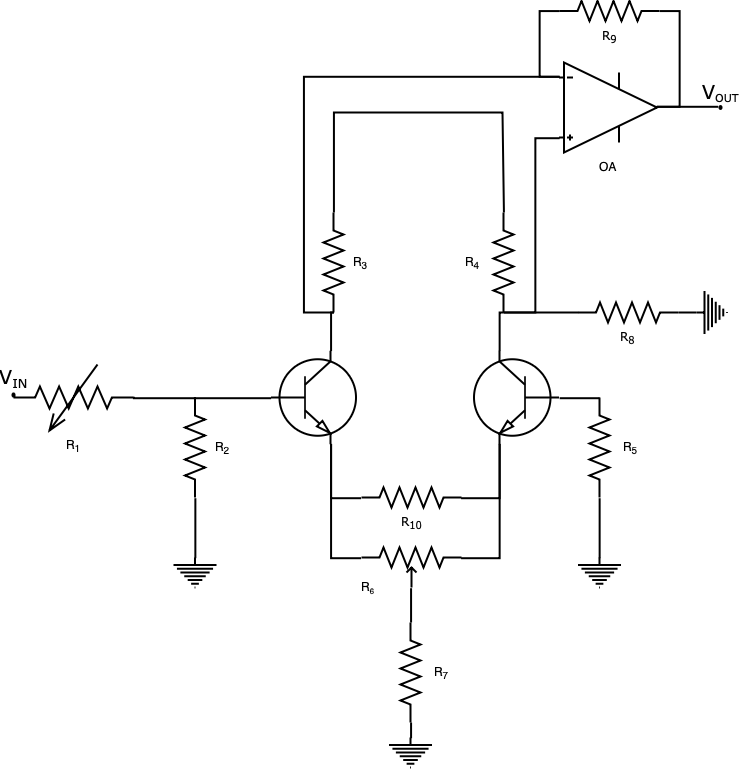
\includegraphics[width=0.5\textwidth]{../Ex3/Resources/conversor.png}
    \caption{Conversor}
    \label{fig:conversor}
    \end{figure}

Para obtener una señal senoidal con la misma amplitud que la entrada, el creador del circuito propone los componentes listados en la Tabla \ref{tab:componentes_conversor}. Los valores de $R_9$ y $R_8$ se seleccionaron de modo que la se obtenga una señal senoidal de amplitud de $1V$ a la salida. 

\begin{table}[h!]
    \centering
    \begin{tabular}{|c|c|}
    \hline
    $R_1$  & $preset- 25k \Omega$ \\ \hline
    $R_2$  & $2.2k\Omega$        \\ \hline
    $R_3$  & $10k \Omega$        \\ \hline
    $R_4$  & $10k\Omega$         \\ \hline
    $R_5$  & $2.2k\Omega$        \\ \hline
    $R_6$  & $preset- 50k \Omega$ \\ \hline
    $R_7$  & $18k \Omega$        \\ \hline
    $R_8$  & $2.2k \Omega$       \\ \hline
    $R_9$  & $2.2k \Omega$       \\ \hline
    $R_{10}$ & $390 \Omega$        \\ \hline
    \end{tabular}
    \caption{Componentes del conversor}
    \label{tab:componentes_conversor}
    \end{table}


Con todas las etapas del circuito hechas es posible realizar la simulación del circuito completo. En la Figura \ref{fig:sim_circuito_completo} se puede ver una simulación del circuito cuando $V_{IN} = 5V$. En dicha figura se puede apreciar tanto el trigger como la triangular y la senoidal. Cabe aclarar que se configuraron $R_1 = 10k \Omega$ y $R_6 = 50k \Omega$ ($25k \Omega$ de cada lado). Nótese que, la curva roja es la tensión $V_{TR}$ que representa la señal triangular mientras que la negra es $V_{out}$ que es la señal senoidal de salida. La simulación resulta ser muy buena. Se obtuvo una señal senoidal con amplitud de aproximadamente $V_{out}= 1.03V$ y $f = 10.256 kHz$

\begin{figure}[h!]                                                       
    \centering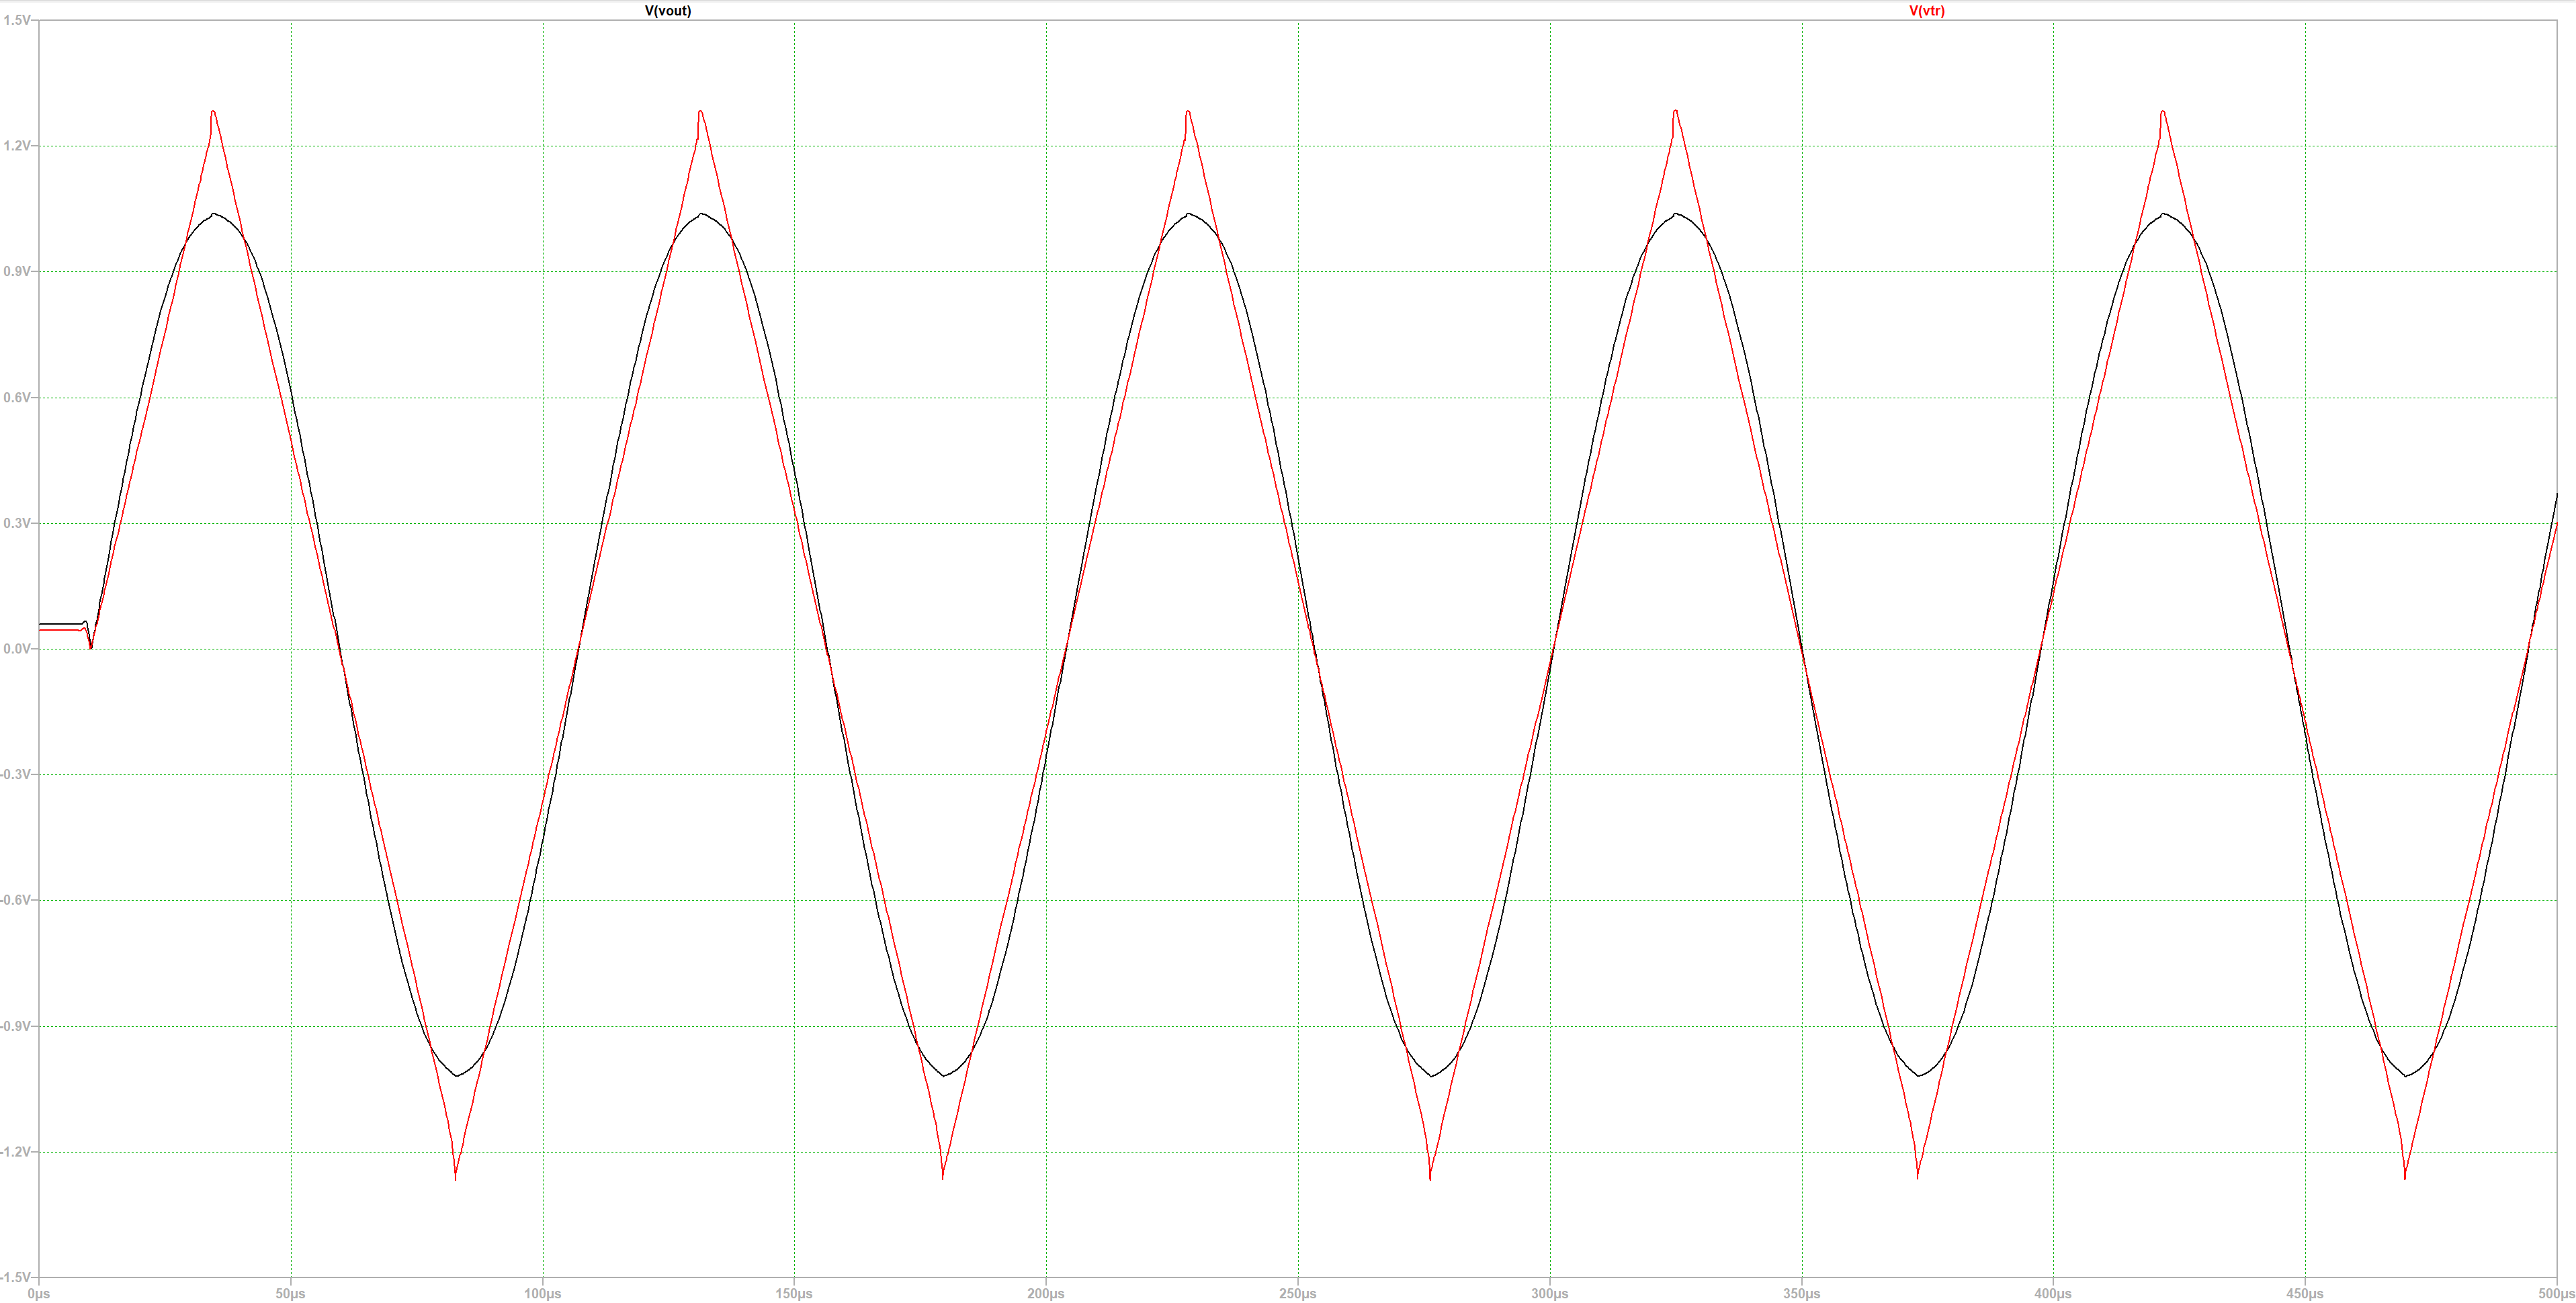
\includegraphics[width=0.9\textwidth]{../Ex3/Resources/sim_completo.png}
    \caption{Simulación del circuito con $V_{in} = 5$}
    \label{fig:sim_circuito_completo}
    \end{figure}


Para terminar la etapa de diseño es de suma importancia notar que el circuito fue diseñado de modo que cuando la $V_{IN} = 5V$ la frecuencia de la senoidal sea $f_0 = 10kHz$ con amplitud $1V$. Esto cumple con los parámetros deseados del $VCO$. Sin embargo, $f_0 = 1kHz$ no se alcanza con $V_{in} = 0V$ sino que con aproximadamente $V_{in} = 0,4 V$. Esta situación se evidencia en la sección \textit{Medición}. Luego, el rango de trabajo del $VCO$ se achica de $[0V;5V]$ a $[0.4V;5V]$. Esto se puede solucionar con una etapa de transformación lineal. Sin embargo, se decide no agregar dicha etapa al diseño ya que los resultados de la simulación fueron satisfactorios. 

Por otro lado, no esta de mas aclarar que, para todas las simulaciones se utilizan el modelo del amplificador operacional TL084 ya que el mismo cuenta con cuatro amplificadores operacionales y el diseño del circuito completo requiere tres. El cuarto amplificador se utiliza en configuración de buffer entre la etapa del $VCO$ y la etapa del conversor. 

\subsection{PCB}
En la Figura \ref{fig:pcb} se muestra el diseno del PCB del circuito propuesto. Notese que se utilizan jumpers de me manera que se pueden desacoplar las etapas del circuito y calibrar las mismas de manera apropiada. Ademas, se utilizan capacitores de desacople de $100nF$ colocados lo mas cerca posible del integrado. 

\begin{figure}[h!]                                                       
    \centering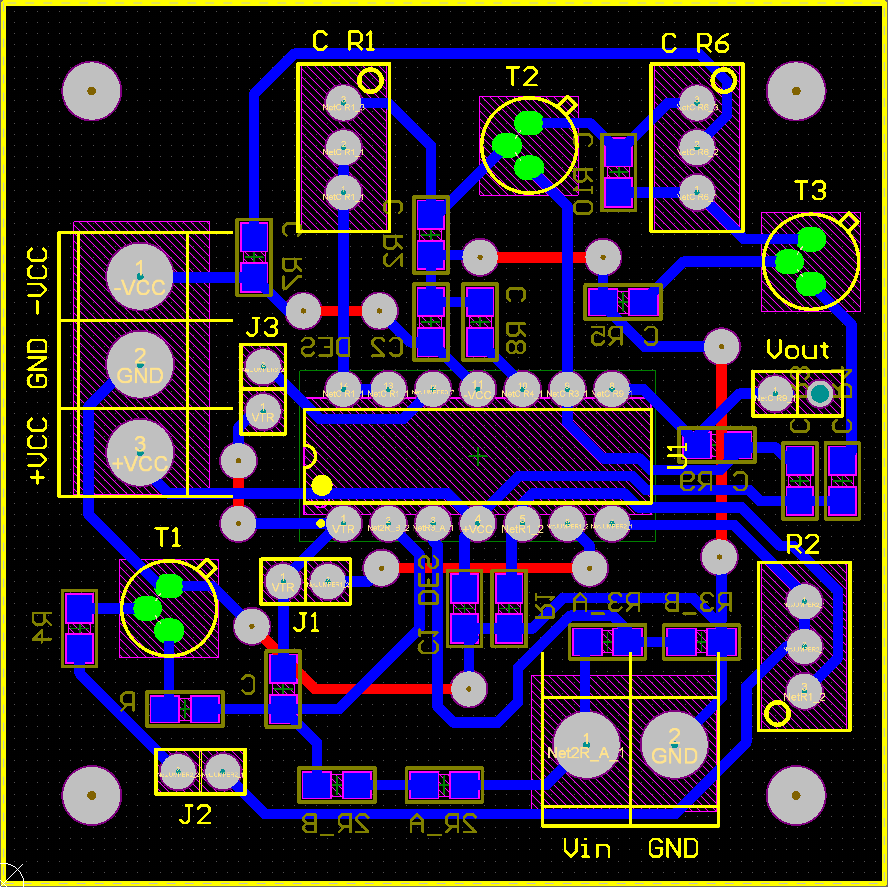
\includegraphics[width=0.5\textwidth]{../Ex3/Resources/pcb.png}
    \caption{Diseño del PCB}
    \label{fig:pcb}
    \end{figure}


\section{Medición}

En esta sección se realizan las mediciones del circuito propuesto en la sección de \textit{Diseño}. Recordar que el circuito cuenta con tres presets para ser calibrado. La forma de calibrar el circuito es la siguiente. En primer lugar,se modifica $R_2$ de la etapa del trigger y se configura para que la frecuencia de la señal triangular se corresponda con $V_{in}$. En segundo lugar, se modifica $R_6$ de la etapa del conversor de modo que la corriente que fluye en la base de los transistores sea la misma. Por ultimo, utilizando la función FET de un osciloscopio se calibra la señal senoidal con $R_1$ de la etapa del conversor. La función FET muestra los armónicos de la señal senoidal. Luego, como la señal senoidal ideal es aquella que tiene solo un armónico principal, se calibra $R_1$ de modo que los armónicos (no el principal) que muestra la función FET sean lo mas chicos posibles. 

\begin{figure}[h!]                                                       
    \centering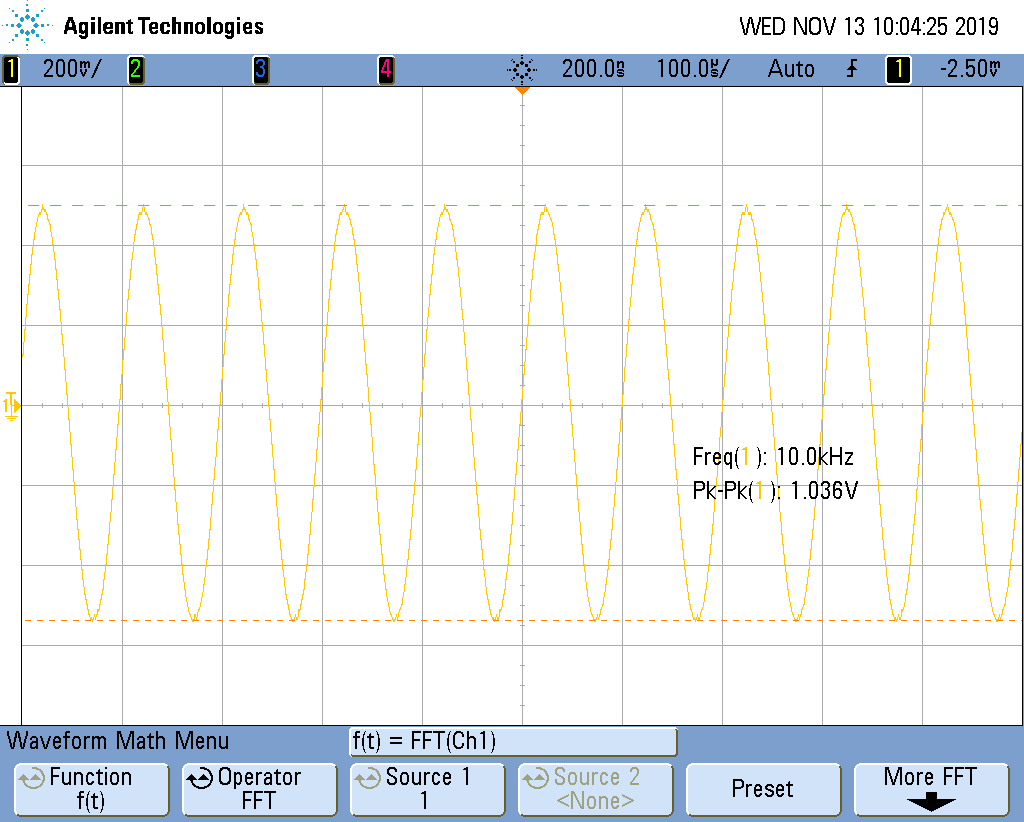
\includegraphics[width=0.9\textwidth]{../Ex3/Resources/med_senoidal_5v.png}
    \caption{Medición con $V_{in} = 5$}
    \label{fig:med_5v}
    \end{figure}

Como medición inicial se configura $V_{IN} = 5V$ y se calibra como se explico anteriormente. En la Figura \ref{fig:med_5v} se ve la medición. Como se puede apreciar los resultados son satisfactorios. La amplitud de la senoidal es $1.036V$ lo que es muy próximo a $1V$. Entonces, se concluye que se logro la amplitud deseada. Ademas, la frecuencia es $10kHz$ que es la deseada. 

Se continua a medir el \textit{jitter}. Para hacerlo, se vario $V_{in}$ y se medio la frecuencia de la señal senoidal con mediciones estadísticas mayores a $20k$. En la Tabla \ref{tab:medicion_jitter} se pueden ver dichas mediciones. Como se puede ver, en todos los casos la desviación standard resulto ser de tres ordenes de magnitud menor que la frecuencia media. Ademas, la diferencia entre la frecuencia máxima y media ronda alrededor de $1\%$ siendo la mejor de $0.23\%$ y la peor de $1.2 \%$. Se puede concluir que los resultados son satisfactorios. Por otro lado, en estas mediciones se manifiesta la relación lineal que existe entre $V_{in}$ y la frecuencia de la senoidal. Ademas, como se anticipo, se obtiene una frecuencia de $f = 1kHz$ cuando $V_{in} = 0.464 V$. 

% Please add the following required packages to your document preamble:
% \usepackage{booktabs}
\begin{table}[]
    \centering
    \begin{tabular}{@{}cccccc@{}}
    \toprule
    $V_{in}$ (V) & f media (kHz) & f mínima (kHz) & f máxima (kHz) & Desv std (Hz) & Count (k) \\ \midrule
    5            & 9.989         & 9.94           & 10.06          & 11.434        & 30.16     \\
    4            & 8.1610        & 8.13           & 8.20           & 8.862         & 20.11     \\
    3            & 6.252         & 6.23           & 6.27           & 6.658         & 20.13     \\
    2            & 4.259         & 4.25           & 4.26           & 0.706         & 20.12     \\
    1            & 2.160         & 2.15           & 2.16           & 1.884         & 20.08     \\
    0.464        & 0.999         & 0.99           & 1.00           & 0.739         & 20.1      \\ \bottomrule
    \end{tabular}
    \caption{Medición de \textit{Jitter} para distintos valores de $V_{in}$}
    \label{tab:medicion_jitter}
    \end{table}

Como se dijo anteriormente, se mide el $THD$ mediante el osciloscopio tomando los primeros 5 armónicos. En la Tabla \ref{tab:medicion_thd} se pueden ver dichas mediciones. Como se puede ver, en todas las mediciones el $THD$ resulto ser menor del $2\%$. Recordar que, este parámetro depende de la precision de la calibración del circuito el cual puede varar mucho. Ademas, depende del circuito de la etapa del conversor que contiene transistores. Al contener transistores, puede que la temperatura de los mismos difiera entra cada medición agregando error a las mediciones. Cabe aclarar que, también, se utilizo el analizador de espectros de audio para realizar las mediciones. Si bien este dispositivo computa el parámetro $THD$ mas rápido y con mas armónicos, no se pudo obtener una medición clara ya que el valor mostrado variaba entre un numero significante de valores. 


% Please add the following required packages to your document preamble:
% \usepackage{booktabs}
\begin{table}[!h]
    \centering
    \begin{tabular}{@{}ccl@{}}
    \toprule
    $V_{in}$ (V) & Frecuencia fundamental (kHz) & THD $(\%)$ \\ \midrule
    5            & 9.9                          & 1.44       \\
    4            & 8.1                          & 1.64       \\
    3            & 6.1                          & 1.41       \\
    2            & 4.1                          & 1.31       \\
    1            & 2.1                          & 1.17       \\
    0.47         & 1                            & 1.09       \\ \bottomrule
    \end{tabular}
    \caption{Medición de $THD$}
    \label{tab:medicion_thd}
    \end{table}

\section{Conclusión}
Se logro diseñar e implementar un $VCO$ con una salida senoidal de $1V$ de amplitud con un rango de frecuencias de $[1kHz; 10kHz]$. Si bien el rango de trabajo se vio acotado a $[0.47V;5V]$ se logro obtener los parámetros de \textit{jitter} y $THD$ dentro de los rangos deseados. Como consideraciones adicionales se podría implementar una etapa de trasformación lineal para ajustar el rango de trabajo del $VCO$. Ademas, se podrían evaluar otros transistores para mejorar la etapa conversora y asi mejorar los parámetros de \textit{jitter} y $THD$. 




